\documentclass[10pt, a4paper]{scrartcl}

\usepackage{vorschule}
\usepackage[
	typ=ab,
	fach=Informatik,
	lerngruppe={Q1-LK} ,
	nummer=4,
	module={Symbole,Lizenzen},
	seitenzahlen=keine,
	farbig,
	lizenz=cc-by-nc-sa-4,
]{schule}

\usepackage[
	kuerzel=Ngb,
	reihe={Automaten und formale Sprachen} ,
	version={2021-03-03} ,
]{ngbschule}

\author{J. Neugebauer}
\title{Mealy-Automaten}
\date{\Heute}

\setzeAufgabentemplate{ngbnormal}


\begin{document}
\ReiheTitel

Ein \textbf{Mealy-Automat} ist ein Automat, der für jeden Übergang nicht nur eine Eingabe aus dem \emph{Eingabealphabet} festlegt, sondern auch eine Ausgabe aus einem \emph{Ausgabealphabet}.

Ein Mealy-Automat wird als 6-Tupel $A = (Q, \Sigma, \Omega, \delta, \lambda, q_0)$ definiert:
\begin{itemize}
	\item $Q$ ist die (endliche) Menge von Zuständen des Automaten.
	\item $\Sigma$ ist das Eingabealphabet.
	\item $\Omega$ ist das Ausgabealphabet.
	\item $\delta: Q\times \Sigma\rightarrow Q$ ist die Übergangsfunktion.
	\item $\lambda: \Omega\times \Sigma\rightarrow \Omega$ ist die Ausgabefunktion.
	\item $q_0\in Q$ ist der Startzustand.
\end{itemize}

(Beachte, dass es keinen Endzustand gibt. Ein Mealy-Automat akzeptiert also keine Worte, sondern erzeugt zu einem Wort eine Ausgabe.)

\begin{aufgabe}
	Konstruiere den gezeigten Mealy-Automaten in FLACI und teste ihn. Was macht der Automat?
	
	\begin{figure}[h]\centering
		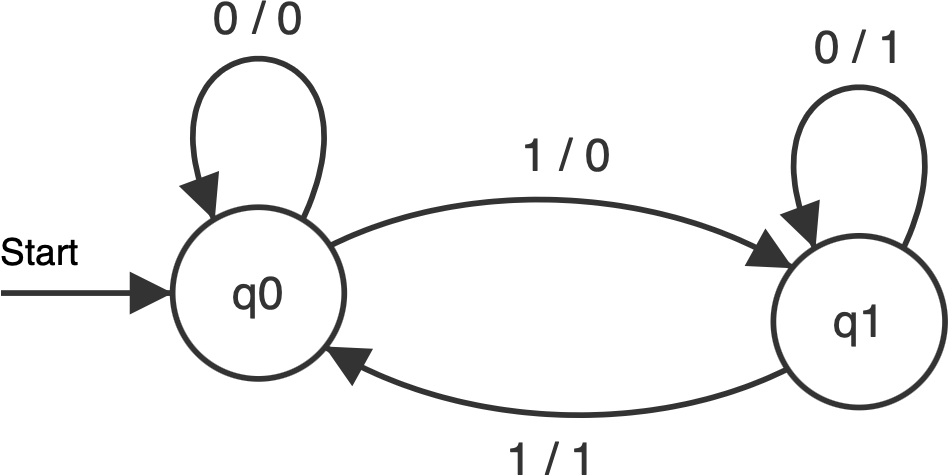
\includegraphics[width=6cm]{Q1-LK-AB.4-Abb_Mealy_1}
		\caption{Ein Mealy-Automat}
	\end{figure}
\end{aufgabe}

\begin{aufgabe}
	Konstruiere in FLACI einen Mealy-Automaten mit dem Eingabealphabet $\Sigma = \{ 0, 1, 2, 3 \}$ und dem Ausgabealphabet $\Omega = \{ 0, 1, 2, 3, 4, 5, 6 \}$, der für Eingaben aus zwei Buchstaben (z.B. $23$) die Summe der Zahlen bestimmt (also hier $05$).
	
	\tipp{Es reichen sechs Zustände zur Umsetzung des Automaten.}
\end{aufgabe}

\end{document}